\documentclass[10pt, a4paper]{article}

\usepackage{ctex}
\usepackage{xeCJK}
\usepackage{caption}
\usepackage{geometry}
\geometry{
    left = 0.6in,
    right = 0.6in,
    top = 0.8in,
    bottom = 1.0in
}
\usepackage{amssymb}
\usepackage{amsbsy}
\usepackage{amsmath}
\usepackage{xcolor}
\usepackage{mathrsfs}
\usepackage{graphicx}
\usepackage{pifont}
\usepackage{tasks}
\settasks{
    label = \Alph*. ,
    label-width = 16pt
}
\pagestyle{empty}

\newcommand{\Title}[3]{
    \begin{center}
        \Large \textbf{中国电子学会 #1~年~#2~月 Scratch~#3级考试}
    \end{center}
}
\newcommand{\TimeAndName}[1]{
    \begin{center}
        考试时间:~#1~ 分钟 \qquad\qquad\qquad\qquad 姓名:\underline{\quad\quad\quad\quad}
    \end{center}
}

\begin{document}
    \Title{2022}{9}{一} % 标题
    \TimeAndName{60} % 考试时间及姓名

    % 单选题
    \vspace{2mm}
    {\noindent\textbf{第一部分、单选题(共 25 题,每题 2 分,共50分.)}}
    \begin{enumerate}
        % 1
        \item 点击绿旗,下列哪个选项可以实现播放马叫声并在声音全部播放完后,马向右移动?(\qquad)
        \begin{center}
            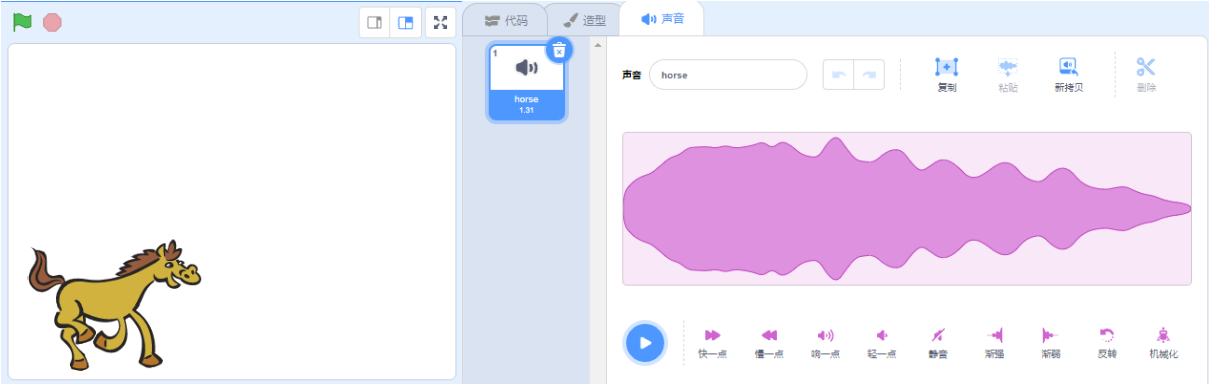
\includegraphics[width=.8\textwidth]{1.png}
        \end{center}
        \begin{tasks}(4)
            \task 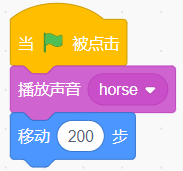
\includegraphics[width=.15\textwidth]{1a.png}
            \task 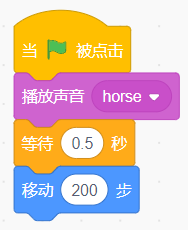
\includegraphics[width=.12\textwidth]{1b.png}
            \task 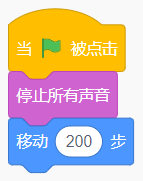
\includegraphics[width=.12\textwidth]{1c.png}
            \task 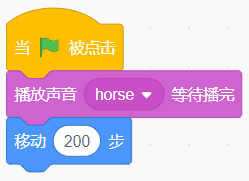
\includegraphics[width=.18\textwidth]{1d.png}
        \end{tasks}

        % 2
        \item 如图所示,角色Ben运行下一个造型积木,下列说法不正确的是?(\qquad)
        \begin{tasks}
            \task 若当前造型为“ben-a”,则下一个造型为“ben-b”
            \task 若当前造型为“ben-b”,则下一个造型为“ben-c”
            \task 若当前造型为“ben-c”,则下一个造型为“ben-d”
            \task 若当前造型为“ben-d”,则下一个造型仍为“ben-d”
        \end{tasks}

        % 3
        \item 如图所示,把电脑上的一张图片上传到角色列表区,应该用哪个按钮?(\qquad)
        \begin{tasks}(4)
            \task \ding{172}
            \task \ding{173}
            \task \ding{174}
            \task \ding{175}
        \end{tasks}

        % 4
        \item 如图所示,点击绿旗,下列说法正确的是?(\qquad)
        \begin{tasks}
            \task 不会播放任何声音
            \task 点击绿旗,等待1秒后,会播放“喵”的声音
            \task 点击绿旗,“喵”的声音刚开始播放就瞬间没有了
            \task 点击绿旗,等待1秒后,“喵”的声音刚开始播放就瞬间没有了
        \end{tasks}

        \begin{figure}[htbp]
            \centering
            \begin{minipage}[t]{.15\textwidth}
                \centering
                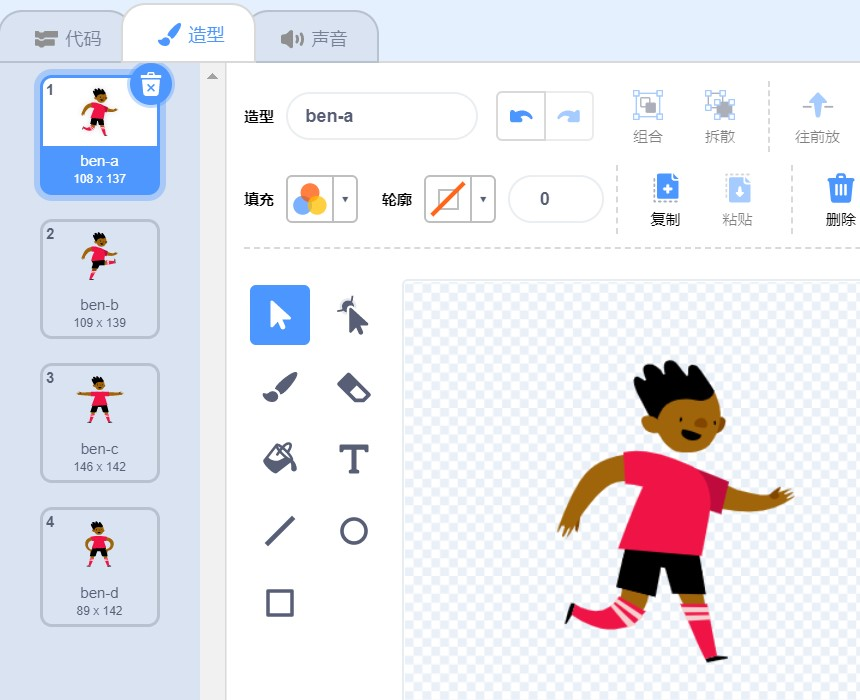
\includegraphics[width=\textwidth]{2.jpg}
                \caption*{第 2 题}
            \end{minipage}
            \begin{minipage}[t]{.1\textwidth}
                \centering
                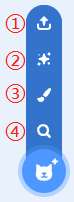
\includegraphics[width=.45\textwidth]{3.png}
                \caption*{第 3 题}
            \end{minipage}
            \begin{minipage}[t]{.3\textwidth}
                \centering
                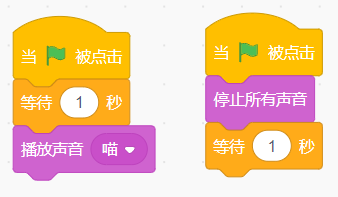
\includegraphics[width=.7\textwidth]{4.png}
                \caption*{第 4 题}
            \end{minipage}
            \begin{minipage}[t]{.2\textwidth}
                \centering
                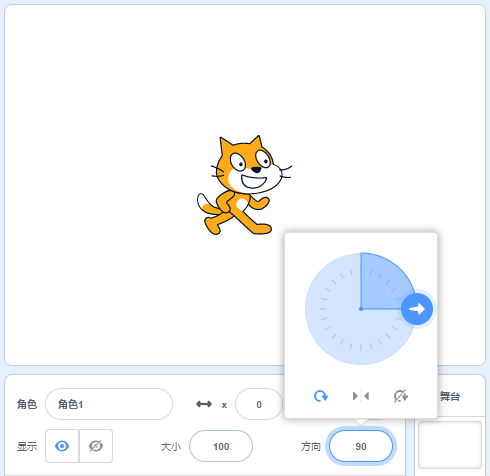
\includegraphics[width=.6\textwidth]{5.png}
                \caption*{第 5 题}
            \end{minipage}
        \end{figure}

        % 5
        \item 如图所示,默认小猫角色,下列哪个选项能让小猫面朝下方?(\qquad)
        \begin{tasks}(4)
            \task 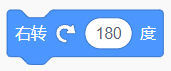
\includegraphics[width=.12\textwidth]{5a.png}
            \task 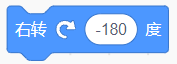
\includegraphics[width=.12\textwidth]{5b.png}
            \task 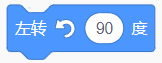
\includegraphics[width=.12\textwidth]{5c.png}
            \task 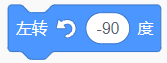
\includegraphics[width=.12\textwidth]{5d.png}
        \end{tasks}

        \newpage
        % 6
        \item 当前造型为“ben-a”, 下列哪个选项不能将角色Ben切换成“ben-d”造型?(\qquad)
        \begin{tasks}(4)
            \task 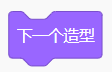
\includegraphics[width=.1\textwidth]{6a.png}
            \task 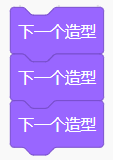
\includegraphics[width=.06\textwidth]{6b.png}
            \task 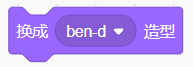
\includegraphics[width=.15\textwidth]{6c.png}
            \task 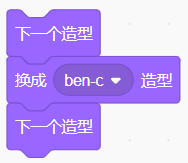
\includegraphics[width=.1\textwidth]{6d.png}
        \end{tasks}

        % 7
        \item 关于舞台背景,下列选项正确的是?(\qquad)
        \begin{tasks}(4)
            \task 不可使用运动类积木
            \task 不可使用外观类积木
            \task 不可使用声音类积木
            \task 不可对背景进行编程
        \end{tasks}

        % 8
        \item 背景如下图所示,下列选项正确的是?(\qquad)
        \begin{tasks}
            \task 当删除背景编号为1的背景后,剩下的背景编号分别为2、3、4、5
            \task 在角色代码中不能切换舞台背景
            \task 如果当前背景为“Blue Sky”,执行“下一个背景”积木后,背景不会发生切换
            \task 无法删除所有背景,至少要有1个背景
        \end{tasks}

         \begin{figure}[htbp]
            \centering
            \begin{minipage}[t]{.25\textwidth}
                \centering
                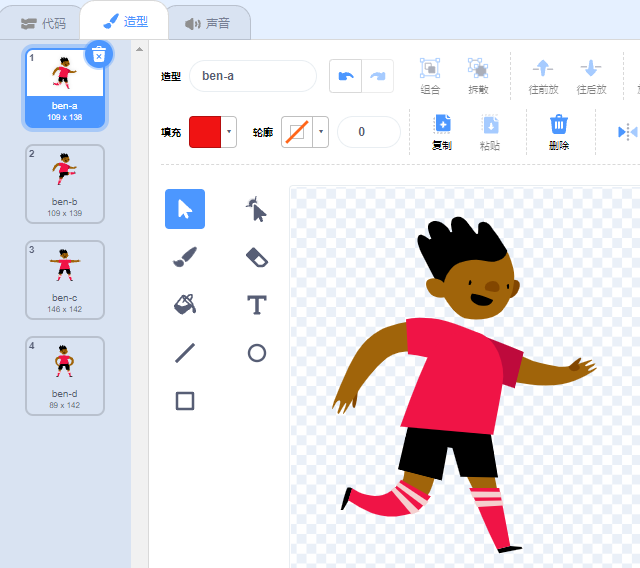
\includegraphics[width=\textwidth]{6.png}
                \caption*{第 6 题}
            \end{minipage}
            \begin{minipage}[t]{.18\textwidth}
                \centering
                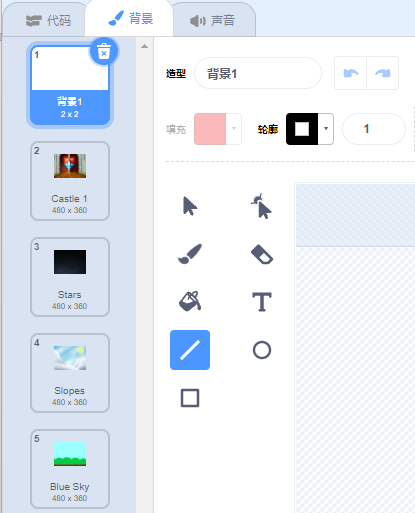
\includegraphics[width=\textwidth]{8.png}
                \caption*{第 8 题}
            \end{minipage}
            \begin{minipage}[t]{.195\textwidth}
                \centering
                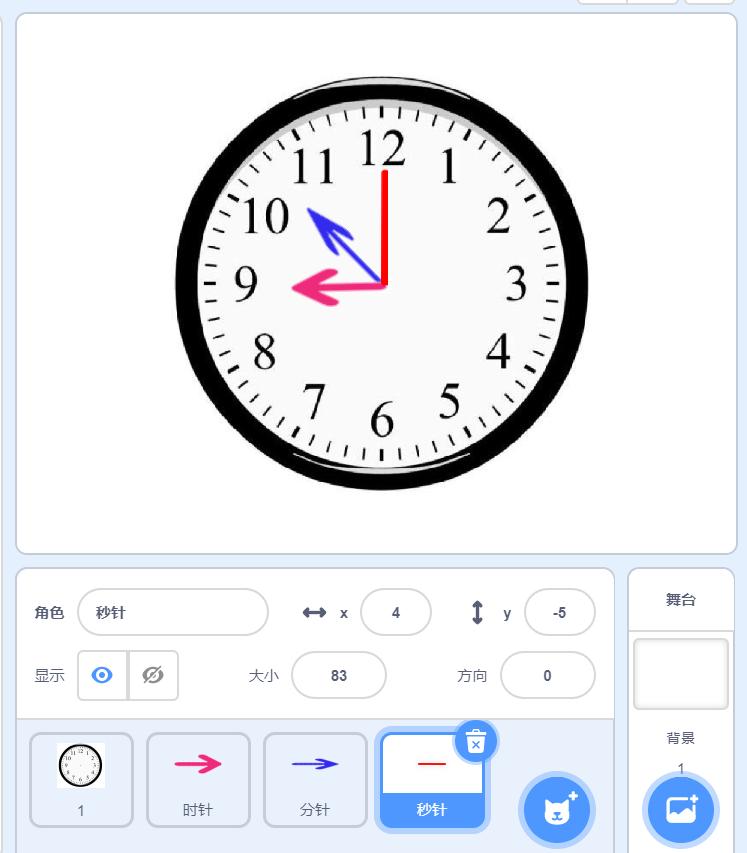
\includegraphics[width=\textwidth]{9.png}
                \caption*{第 9 题}
            \end{minipage}
        \end{figure}

        % 9
        \item 秒针的初始方向如上图所示,秒针中心点在最左端,下列哪个选项可以使秒针指向三点钟方向?(\qquad)
        \begin{tasks}(4)
            \task 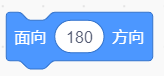
\includegraphics[width=.13\textwidth]{9a.png}
            \task 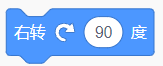
\includegraphics[width=.13\textwidth]{9b.png}
            \task 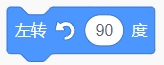
\includegraphics[width=.13\textwidth]{9c.png}
            \task 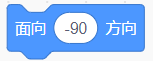
\includegraphics[width=.13\textwidth]{9d.png}
        \end{tasks}

        % 10
        \item 下列选项中哪个积木的运行结果为10?(\qquad)
        \begin{tasks}(4)
            \task 
\includegraphics[width=.13\textwidth]{10a.png}
            \task 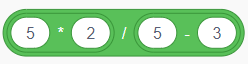
\includegraphics[width=.18\textwidth]{10b.png}
            \task 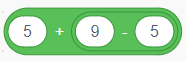
\includegraphics[width=.13\textwidth]{10c.png}
            \task 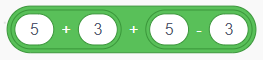
\includegraphics[width=.18\textwidth]{10d.png}
        \end{tasks}

        % 11
        \item 小明拿着10元钱去买水果,买了1个苹果和2个香蕉,结果剩3元,请问1个苹果可能卖多少钱?(苹果和香蕉的单价都是整数)?(\qquad)
        \begin{tasks}(4)
            \task 2元
            \task 3元
            \task 4元
            \task 7元
        \end{tasks}

        % 12
        \item 冬奥会比赛中,某项比赛需进行两轮,各选手两轮得分相加最高者才能赢得冠军。第一轮比赛中,选手甲落后选手乙10分,选手丙落后选手甲5分,选手丁领先选手丙5分;第二轮比赛中,选手甲和选手丁得分反超选手乙5分,选手丙与选手乙得分相同。请问,最终谁拿到了冠军?(\qquad)
        \begin{tasks}(4)
            \task 选手甲
            \task 选手乙
            \task 选手丙
            \task 选手丁
        \end{tasks}

        % 13
        \item 在绘制角色时,选择画圆工具后,须同时按下键盘上的哪个键,才能绘制出正圆?(\qquad)
        \begin{tasks}(4)
            \task Ctrl
            \task Shift
            \task Alt
            \task 空格键
        \end{tasks}
        
        % 14
        \item 点击绿旗后,舞台上将出现什么样的图案?(\qquad)
        \begin{tasks}(4)
            \task 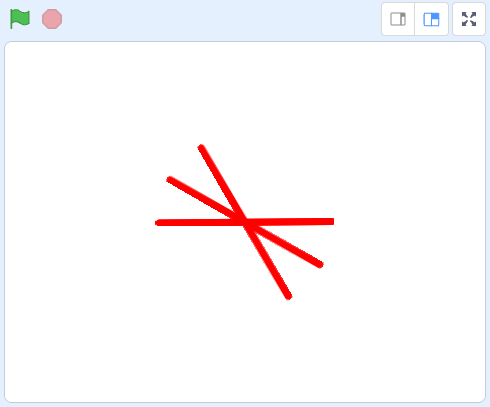
\includegraphics[width=.13\textwidth]{14a.png}
            \task 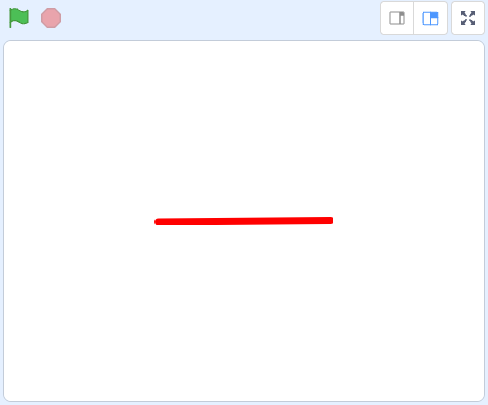
\includegraphics[width=.13\textwidth]{14b.png}
            \task 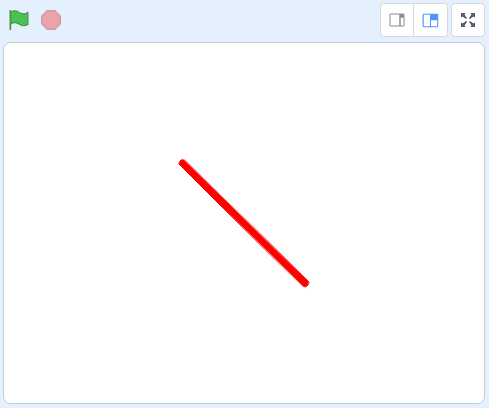
\includegraphics[width=.13\textwidth]{14c.png}
            \task 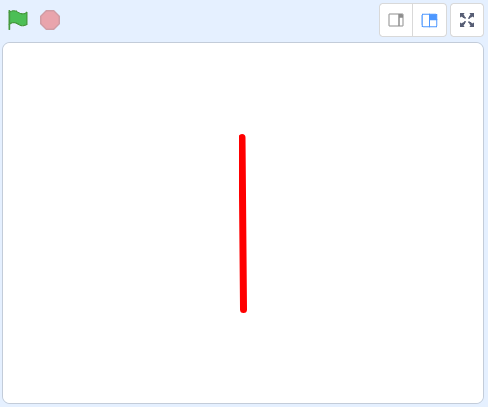
\includegraphics[width=.13\textwidth]{14d.png}
        \end{tasks}

        % 15
        \item 如图所示,角色列表区里有4个角色,可在舞台区只能看到其中的3个,你觉得下列选项中最合理的是?(\qquad)
        \begin{tasks}(2)
            \task 背景太暗,看不清楚
            \task 角色2被删除了
            \task 角色2设置成了“隐藏”
            \task 角色2被背景挡住了
        \end{tasks}

        % 16
        \item 保存图中所示的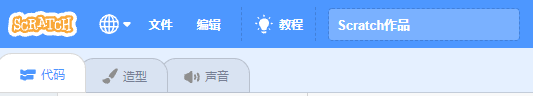
\includegraphics[width=.3\textwidth]{16.png}Scratch作品,不修改作品名字,生成的文件名是?(\qquad)
        \begin{tasks}(4)
            \task Scratch.sb3
            \task Scratch.sprite3
            \task Scratch作品.svg
            \task Scratch作品.sb3
        \end{tasks}

        \begin{figure}[htbp]
            \centering
            \begin{minipage}[t]{.25\textwidth}
                \centering
                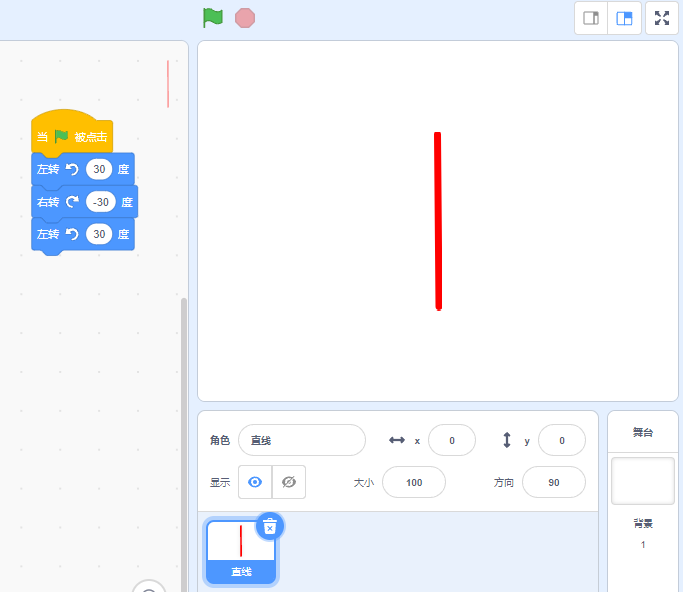
\includegraphics[width=\textwidth]{14.png}
                \caption*{第 14 题}
            \end{minipage}
            \begin{minipage}[t]{.25\textwidth}
                \centering
                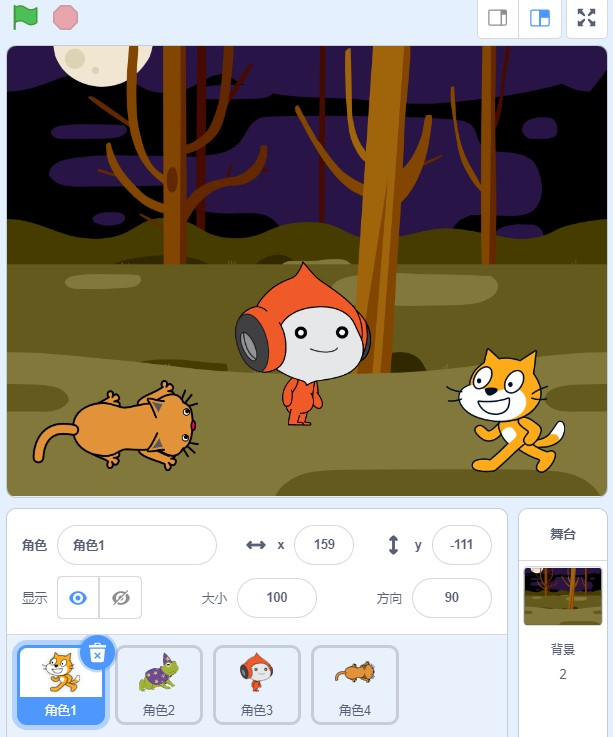
\includegraphics[width=\textwidth]{15.jpg}
                \caption*{第 15 题}
            \end{minipage}
            \begin{minipage}[t]{.28\textwidth}
                \centering
                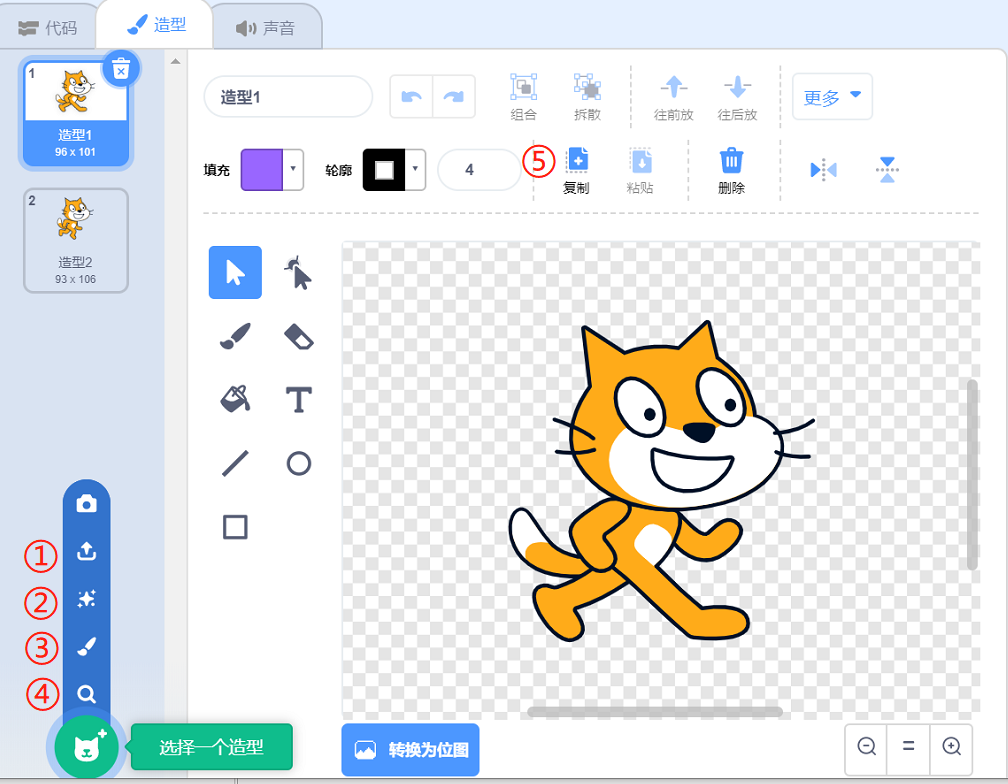
\includegraphics[width=\textwidth]{18.png}
                \caption*{第 18 题}
            \end{minipage}
        \end{figure}

        % 17
        \item 	
        点击全屏模式后,下列哪个选项可以退出全屏模式?(\qquad)
        \begin{tasks}(2)
            \task 按下键盘Esc键或点击
\includegraphics[width=.03\textwidth]{17-1.png}
            \task 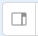
\includegraphics[width=.03\textwidth]{17-2.png}或
\includegraphics[width=.03\textwidth]{17-1.png}
            \task 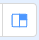
\includegraphics[width=.03\textwidth]{17-3.png}或
\includegraphics[width=.03\textwidth]{17-1.png}
            \task 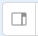
\includegraphics[width=.03\textwidth]{17-2.png}或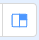
\includegraphics[width=.03\textwidth]{17-3.png}
        \end{tasks}

        % 18
        \item 下列哪个选项不能为小猫添加更多的造型?(\qquad)
        \begin{tasks}
            \task 在“造型1”上点右键,在随后出现的菜单中点“复制”
            \task 在“造型2”上点右键,在随后出现的菜单中点“复制”
            \task 点击图中标注\ding{172}\ding{173}\ding{174}\ding{175}中的任一选项
            \task 点击图中标注\ding{176}的“复制”按钮
        \end{tasks}

        % 19
        \item 关于小猫的声音,下列说法不正确的是?(\qquad)
        \begin{tasks}(2)
            \task 我们可以为小猫添加更多的声音,甚至是狗叫声
            \task 我们可以为小猫录制一段声音
            \task 小猫角色中默认包含了名称为“喵”的声音
            \task 我们只能为小猫添加声音库中的声音
        \end{tasks}

        % 20
        \item 下列哪个选项不是“清除音效”积木的作用?(\qquad)
        \begin{tasks}(2)
            \task 将“音调”恢复成默认值
            \task 将“音量”恢复成默认值
            \task 将“左右平衡”恢复成默认值
            \task 同时将“音调”和“左右平衡”恢复成默认值
        \end{tasks}

        \newpage
        % 21
        \item 小猫位置如图所示,下列哪个选项可以让小猫到达小球的位置?(\qquad)
        \begin{tasks}(4)
            \task 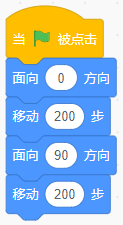
\includegraphics[width=.11\textwidth]{21a.png}
            \task 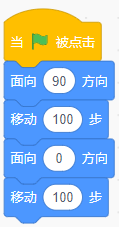
\includegraphics[width=.11\textwidth]{21b.png}
            \task 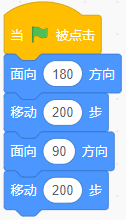
\includegraphics[width=.12\textwidth]{21c.png}
            \task 
\includegraphics[width=.12\textwidth]{21d.png}
        \end{tasks}

        % 22
        \item 在多个背景的情况下,下列哪个选项可以实现:当点击角色时,角色回答当前背景的编号?(\qquad)
        \begin{tasks}(4)
            \task 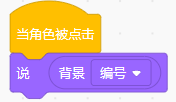
\includegraphics[width=.15\textwidth]{22a.png}
            \task 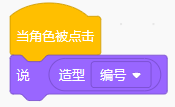
\includegraphics[width=.15\textwidth]{22b.png}
            \task 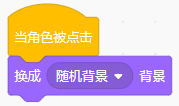
\includegraphics[width=.15\textwidth]{22c.png}
            \task \includegraphics[width=.15\textwidth]{22d.png}
        \end{tasks}

        \begin{figure}[htbp]
            \centering
            \begin{minipage}[t]{.2\textwidth}
                \centering
                \includegraphics[width=\textwidth]{21.png}
                \caption*{第 21 题}
            \end{minipage}
            \begin{minipage}[t]{.35\textwidth}
                \centering
                \includegraphics[width=\textwidth]{25.jpg}
                \caption*{第 25 题}
            \end{minipage}
        \end{figure}

        % 23
        \item 下列选项说法正确的是?(\qquad)
        \begin{tasks}
            \task 不能在背景的程序里,控制角色造型的切换
            \task 只能切换到下一个背景,不能切换到上一个背景
            \task “当角色被点击”积木属于“控制”类积木
            \task 假如一个作品中有多个角色,我们可以在某一角色的程序里控制其它角色的造型切换
        \end{tasks}

        % 24
        \item 角色包含多个造型,下列说法正确的是?(\qquad)
        \begin{tasks}(2)
            \task 所有造型都是不可修改的
            \task 所有造型都是可以修改的
            \task 只能修改其中一个造型
            \task 不可以自拍一张图片作为新造型
        \end{tasks}

        % 25
        \item 龙舟赛是我国传统节日端午节的主要民俗活动。龙舟船尾处绘制有绿色的吃水线标志,吃水线有4个刻度(如图所示吃水线里的4条绿色横线),由上到下分别标记了\ding{172}、\ding{173}、\ding{174}、\ding{175}符号。龙舟赛有快乐龙舟队、开心龙舟队、团结龙舟队和勇敢龙舟队四支队伍参赛,当快乐龙舟队比赛时,水面与吃水线的\ding{172}号刻度平齐;当团结龙舟队比赛时,水面与吃水线的\ding{173}号刻度平齐;当开心龙舟队比赛时,水面与吃水线的\ding{174}号刻度平齐;当勇敢龙舟队比赛时,水面与吃水线的\ding{175}号刻度平齐。给四支龙舟队按其重量排序,由小到大的顺序应该是?(\qquad)
        \begin{tasks}
            \task 快乐龙舟队,开心龙舟队,团结龙舟队,勇敢龙舟队
            \task 快乐龙舟队,团结龙舟队,开心龙舟队,勇敢龙舟队
            \task 团结龙舟队,勇敢龙舟队,开心龙舟队,快乐龙舟队
            \task 勇敢龙舟队,开心龙舟队,团结龙舟队,快乐龙舟队
        \end{tasks}
    \end{enumerate}

    % 判断题
    \newpage
    {\noindent\textbf{第二部分、判断题(共 10 题,每题 2 分,共20分.)}}
    \begin{enumerate}
        \setcounter{enumi}{25}
        % 26
        \item 一个角色只能包含一个造型。(\qquad)

        % 27
        \item 我们可以根据需要将角色的任意一点设为造型中心。(\qquad)

        % 28
        \item 一个程序只能播放一次声音。(\qquad)

        % 29
        \item 我们在Scratch 默认的白色舞台背景上绘制了一条线段,然后又从背景库中选择了另外一张背景添加到作品中,那这条线段也同时出现在后来添加的背景中。(\qquad)

        \begin{figure}[htbp]
            \centering
            \begin{minipage}[t]{.15\textwidth}
                \centering
                \includegraphics[width=\textwidth]{31.png}
                \caption*{第 31 题}
            \end{minipage}
            \begin{minipage}[t]{.15\textwidth}
                \centering
                \includegraphics[width=\textwidth]{33.png}
                \caption*{第 33 题}
            \end{minipage}
            \begin{minipage}[t]{.15\textwidth}
                \centering
                \includegraphics[width=\textwidth]{34.png}
                \caption*{第 34 题}
            \end{minipage}
            \begin{minipage}[t]{.3\textwidth}
                \centering
                \includegraphics[width=\textwidth]{35.jpg}
                \caption*{第 35 题}
            \end{minipage}
        \end{figure}

        % 30
        \item 黑兔、灰兔和白兔三只兔子比赛跑步。黑免说:“我跑得不是最快的,但比白兔快。”,从这个描述可以得知,黑兔子跑得最快。(\qquad)

        % 31
        \item 执行下列程序,我们将无法听到猫叫声。(\qquad)

        % 32
        \item 我们想打开电脑里存放的一个Scratch文件,可以通过先点击“编辑”菜单,再点击“从电脑中打开”。(\qquad)

        % 33
        \item 对于默认角色小猫,执行下列程序,小猫距离舞台右边缘的距离要大于其距离左边缘的距离。(\qquad)
        
        % 34
        \item 对于角色来说,下列两段程序的运行效果是一样的。(\qquad)

        % 35
        \item 角色造型中的各部分在矢量图模式下默认是拆散的(如下图所示),当点击“转换为位图”后,此时的造型各部分仍是可以拆散的。(\qquad)
    \end{enumerate}

    \newpage
    {\noindent \textbf{第三部分、编程题(共 2 题,共30分.)}}
    \begin{enumerate}
        \setcounter{enumi}{35}
        
        % 36
        \item 踢足球:
        
        1. 准备工作
        \begin{tasks}[label = (\arabic*)]
            \task 选择背景Baseball 2;
            \task 删除默认的小猫角色,选择角色Ben和Soccer Ball。
        \end{tasks}
        2. 功能实现
        \begin{tasks}[label = (\arabic*)]
            \task Ben初始造型为ben-a,初始位置为舞台左下角;
            \task Soccer Ball位于Ben脚前不远处;
            \task 点击绿旗,等哨声(Referee Whistle)结束后,Ben每隔1秒钟切换一个造型,直至其造型为ben-d;
            \task 在切换成ben-b造型后,Soccer Ball往前移动至舞台右边缘;
            \task 观众的欢呼声(Goal Cheer)随即响起,Soccer Ball消失。
        \end{tasks}
        \begin{figure}[htbp]
            \centering
            \begin{minipage}[t]{.3\textwidth}
                \centering
                \includegraphics[width=\textwidth]{36.png}
                \caption*{第 36 题}
            \end{minipage}
            \begin{minipage}[t]{.3\textwidth}
                \centering
                \includegraphics[width=\textwidth]{37.png}
                \caption*{第 37 题}
            \end{minipage}
        \end{figure}

        %37
        \item 猫捉老鼠:
        
        1. 准备工作
        \begin{tasks}[label = (\arabic*)]
            \task 选择背景Witch House;
            \task 删除默认的小猫角色,选择角色Cat 2和Mouse1,Cat 2大小设为80,Mouse1大小设为60。
        \end{tasks}
        2. 功能实现
        \begin{tasks}[label = (\arabic*)]
            \task Cat 2位于舞台左下角,面朝右上(方向55);Mouse1位于舞台右上角,面朝左;
            \task 程序开始,Cat 2边叫边朝向舞台右上角扑去,500步的路程每跑100步就要歇息0.5秒;
            \task 程序开始,Mouse1由舞台右上角跑向舞台左上角,静止不动;
            \task Cat 2扑到舞台右上角落空后,又转向舞台左上角,最终将Mouse1抓住。
        \end{tasks}
    \end{enumerate}
\end{document}